\chapter{Supplemental Information}
\vspace{-0.5em}
\section*{Histogram}
\begin{figure}[h!]
	\centering
	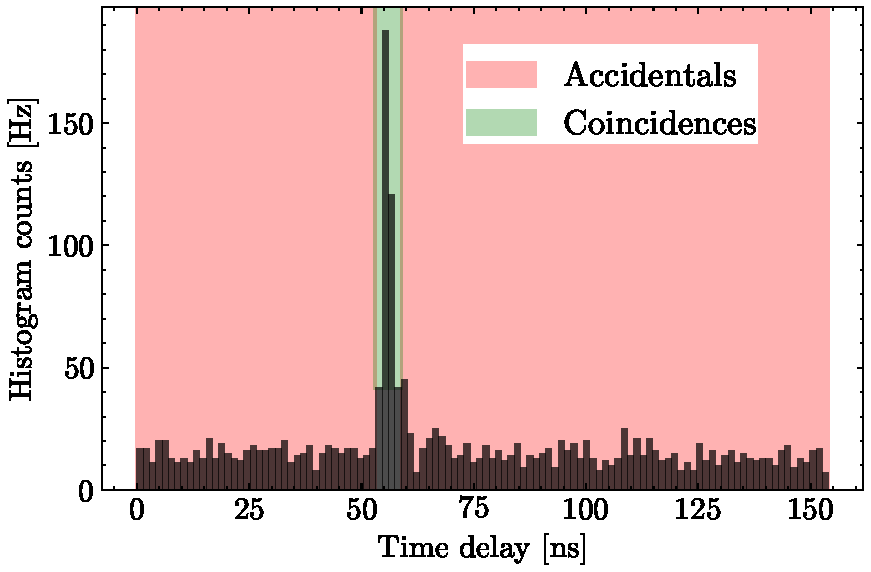
\includegraphics[width=.7\textwidth]{Images/HistogramExample_2.pdf}
	\caption{Representative coincidence histogram using the experimental setup}
	\label{fig:HistExamAcc}
\end{figure}
\vspace{-1.5em}
\section*{Afterpulsing}
\begin{figure}[b!]
	\centering
	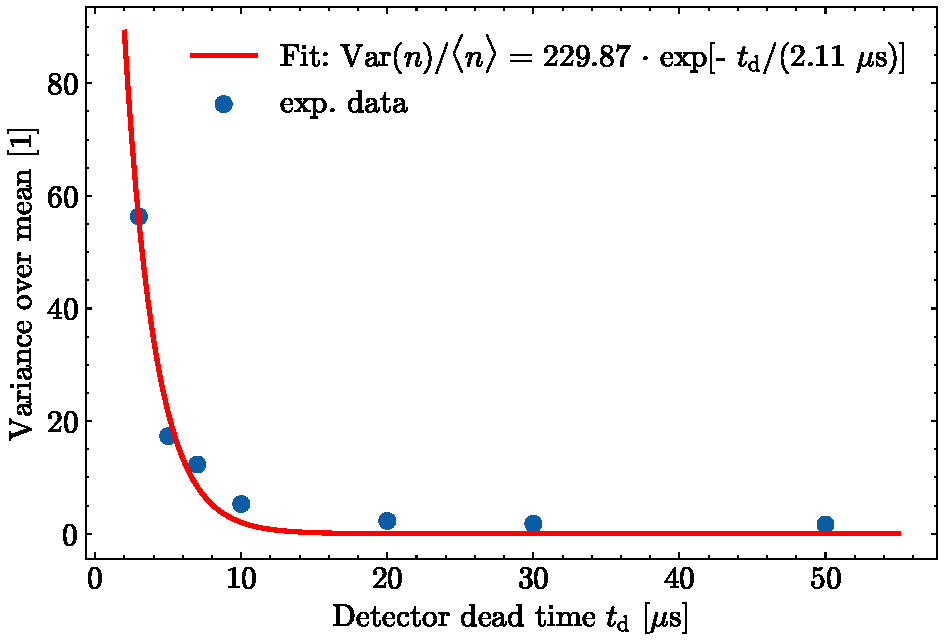
\includegraphics[width=.7\textwidth]{Images/VarMean_DeadTime_Afterpulsing_2.pdf}
	\caption{Variance-to-mean ratio as a function of the dead time of the IR single-photon detector}
	\label{fig:VoMDead}
\end{figure}
\newpage
\section*{Dark counts SNSPD}
\begin{figure}[h!]
	\centering
	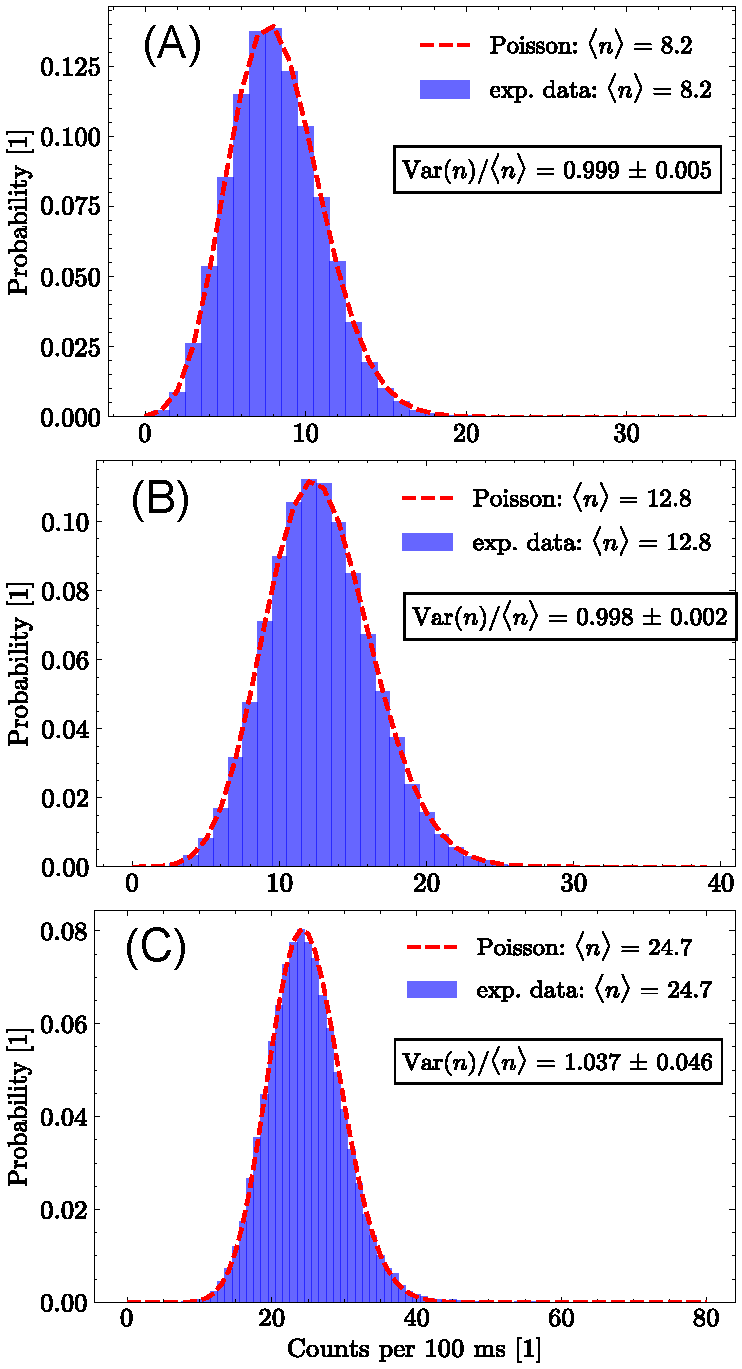
\includegraphics[width=.7\textwidth]{Images/DC_SNSPD_All.pdf}
	\caption{(A): Dark counts in SNSPD channel 2; (B): Dark counts in SNSPD channel 3; (C): Dark counts in SNSPD channel 4}
	\label{fig:DC_SNSPD}
\end{figure}


%\begin{figure}[h!]
%	\noindent
%	\begin{minipage}{0.33\textwidth}
%		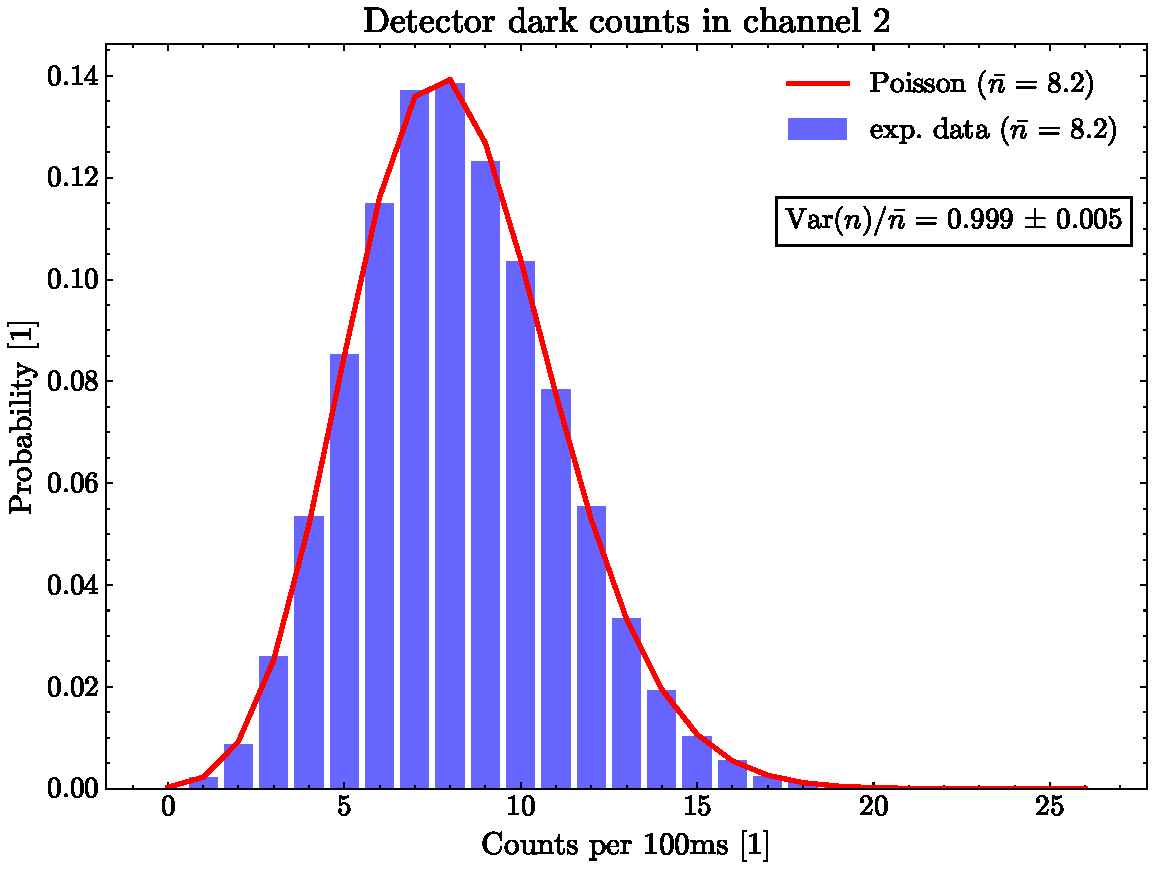
\includegraphics[page=1,width=\linewidth]{Images/DC_chAll.pdf}
%	\end{minipage}%
%	\begin{minipage}{0.33\textwidth}
%		\includegraphics[page=2,width=\linewidth]{Images/DC_chAll.pdf}
%	\end{minipage}%
%	\begin{minipage}{0.33\textwidth}
%		\includegraphics[page=3,width=\linewidth]{Images/DC_chAll.pdf}
%	\end{minipage}
%	\caption{Dark counts of the SNSPD}
%	\label{fig:DC}
%\end{figure}



